% 第3章
\section{CtoCシェアサイクルのサービス設計とビジネスモデル}
  \label{sec:CtoCシェアサイクルのサービス設計とビジネスモデル}
    \par 本研究では,個人所有の余剰自転車を活用し,柔軟かつ地理的制約の少ないシェアサイクル体験を実現するCtoC型のシェアサイクルサービスを提案する.本サービスの最上位コンセプトは,「潜在的リソースを活用して効率化し,モビリティ体験を向上される」ことであり,これにより社会全体の移動効率の向上と資源の有効活用を目指す.本章では,サービス設計,コア技術の活用,及びビジネスモデルの構築について詳述する.
      
  \subsection{サービス設計}
    \label{sec:サービス設計}
      \par 本節では,本研究で提案するサービスの全体像やコンセプトについて紹介する.
      \par まず,本サービスの最上位のコンセプトを一言で表すと,「潜在的リソースを活用して効率化し,モビリティ体験を向上させる」ことにあると考えている.より具体度を上げると,個人が所有している余剰自転車を貸し借りできるプラットフォームを用い,柔軟かつ地理的制約が少ないシェアサイクル体験を実現することに繋がるとも捉えている.
      \par 図を参照しながら本研究で提案するシステムのコンセプトについてより詳しく解説する.図\ref{fig:福井市における既存サービス分布例とCtoCサービスによって期待される分布例}では,福井市内において,福井市より提供されているシェアサイクルサービス「ふくチャリ」の実際の分布例と,CtoCモデルのシェアサイクルサービスが提供されることで期待される分布例を比較している.ふくチャリは,緑色の円でプロットした通り,福井駅を中心とした,福井市内でも比較的人口密度の高い市街などの地域にポートが設置されており,その地域内であればユーザはふくチャリを利用することができる.一方で,海岸線沿いなどの福井市街ではない地域ではポートが設置されていないことが多く,ユーザの需要があった場合でもサービスを提供することが困難である.
      \par そこで,シェアサイクルサービスが設置するポートではなく,個人が所有している自転車の駐輪場に焦点を当てて考えてみると,紫色の円でプロットした通り,多かれ少なかれ地域に差はあれど,地方であっても個人所有の自転車は点在していると想定される.前述したコンセプト「潜在的リソースを活用して効率化し,モビリティ体験を向上させる」で言及している「潜在的リソース」とは,この地方でも変わらず点在している個人所有の自転車を指している.
      \par 提案するサービスやコンセプトを実現するため,本研究で行ったアプローチの全体像は図\ref{fig:CtoCシェアサイクル実現のための本研究のアプローチ全体像}の通りである.シェアサイクルを行うため,NFCまたは指紋認証にて解錠可能なIoTスマートロックや,CtoCモデルにおける効率的なサービス提供を目指した自転車割り当てモデリング,及びそれらを結合するためのインターフェスとなるAPIを構築することで,サービスの提供やコンセプトの実現を目指す.その中で,本研究にて実装を行い,価値提供可能な機能としてはスマートロックの解錠及び施錠のためのプロトタイプと,ここで述べたコンセプトを実現するための,数理最適化による自転車割り当てアルゴリズムである.数理最適化による自転車割り当てアルゴリズムはAPIとして提供し,その中には割り当て処理はもちろんのこと,自転車管理機能などをマイクロサービス設計で実装している.今回実装までは至らなかったものの,決済サービスやスマートロック連携サービスなどの設計も少し行っている.
      \par ユーザエクスペリエンス(UX)の設計の一部であるペルソナは,CtoCシェアリングシステムの貸し手と借り手の二者それぞれについて考える必要がある.なお,ペルソナとは,マーケティングやプロダクト開発などの分野で用いられる,架空の顧客像のことを意味し,典型的なユーザを象徴する人物像を設定する.
      \par 自転車の貸し手として想定しているペルソナをAさんとする.Aさんは都心から少し離れた住宅街に住んでおり,その近くに店舗を構えてカフェを経営している.電動アシスト付き自転車と趣味のロードバイクを1台ずつ保有しているも,自営業であるため忙しく,自転車がほぼオブジェ状態となっている.折角購入したロードバイクがもったいないため,人に貸し出すことができればメンテナンス費用の足しになると考えている.
      \par 自転車の借り手として想定しているペルソナをBさんとする.Bさんも都心から少しはなれた住宅街に住んでいる一人暮らし独身サラリーマンである.平日は電車で会社へ通勤しているため,自転車は保有していない.しかし,自宅から最寄りのコンビニまでは少し距離があり,自転車を利用したいとは思うが,住宅街であるため,BtoCシェアサイクルのステーションが設置されておらず,利用できる自転車がない.
      \par 想定するシチュエーションとしては,このようなAさんとBさんが双方Win-Winの関係で個人間でシェアリングを行うことである.
      \par より身近な別の例として,図\ref{fig:CtoCシェアサイクルの想定されるケーススタディ}のような場合で需要があることが想定される.利用者として示しているある大学生が市役所に行かなければならない用事があるものの,その学生は自転車を所有していないとする.市役所まで徒歩で行けなくもないが,片道30分程度要してしまう距離に位置している.一方で,大学に大量に駐輪されている個人所有者の自転車を利用者が一時的に利用し,市役所まで移動することができれば,片道およそ10分で移動することが可能となる.個人所有者側にも,大学で講義を受けている間に遊休資産となっている自転車を有効活用することができるという観点からメリットがある.
      
      \begin{figure}[htbp]
        \centering
        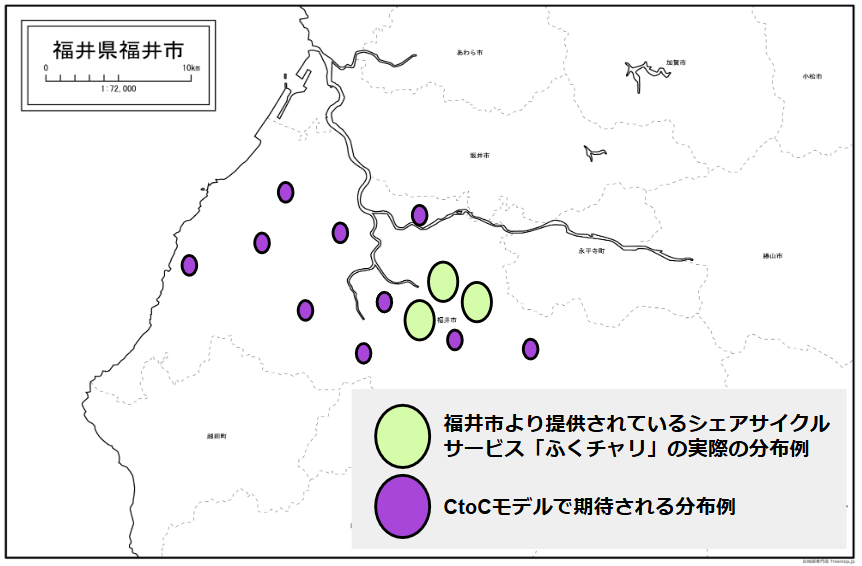
\includegraphics[scale=0.35]
        {figures/mappingExplain.png}
        \caption{福井市における既存サービス分布例とCtoCサービスによって期待される分布例}
        \label{fig:福井市における既存サービス分布例とCtoCサービスによって期待される分布例}
      \end{figure}

      \begin{figure*}[htbp]
        \centering
        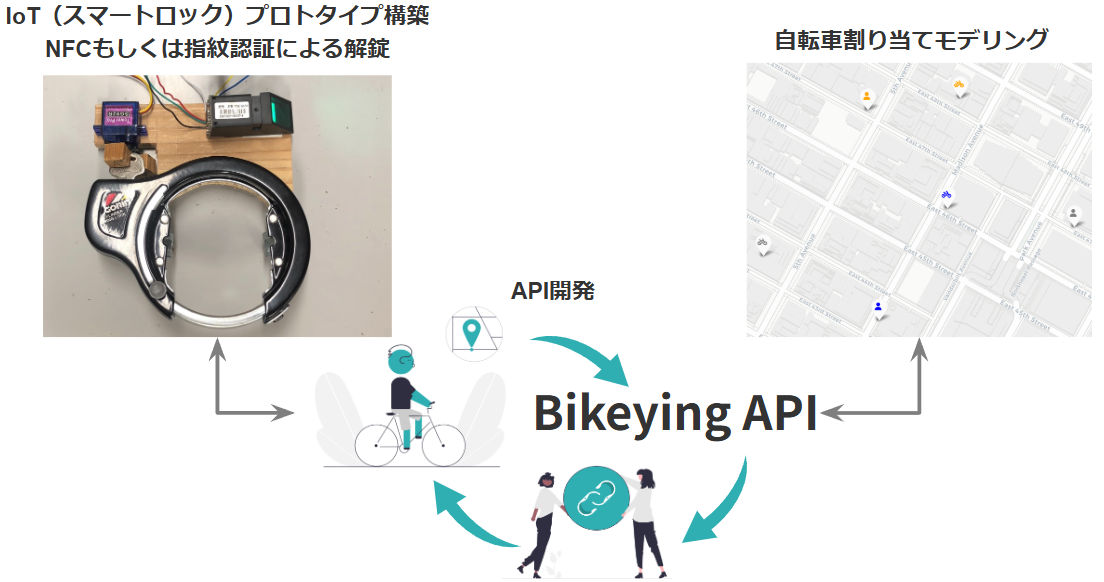
\includegraphics[scale=0.58]
        {figures/approach.png}
        \caption{CtoCシェアサイクル実現のための本研究のアプローチ全体像}
        \label{fig:CtoCシェアサイクル実現のための本研究のアプローチ全体像}
      \end{figure*}

      \begin{figure}[htbp]
        \centering
        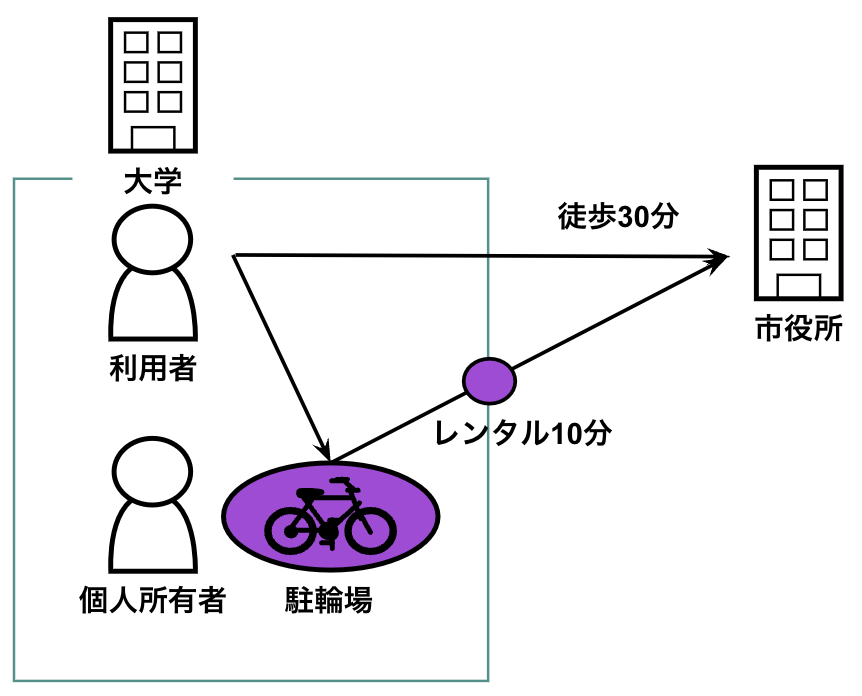
\includegraphics[scale=0.52]
        {figures/casestudy.png}
        \caption{CtoCシェアサイクルの想定されるケーススタディ}
        \label{fig:CtoCシェアサイクルの想定されるケーススタディ}
      \end{figure}
  
  \subsection{コア技術の活用}
    \label{sec:コア技術の活用}
      \par 本節では,本研究を通して活用しているコアな技術について紹介する.
      \par まず,スマートロックに関連する技術について紹介する.これは,大きなくくりではIoT技術と言える.その構成要素として主に,ハードウェア,セキュリティ,及び通信プロトロコルが挙げられる.
      \par ハードウェアでは,ロックの施錠・解錠を自動化するための小型電動モータであるサーボモータや,ロックを解錠するトリガーとなる指紋認証センサ,スマートフォンに内蔵されているNFC(Near Field Communication)リーダを利用している.また,それらを統合するめにマイコンを利用している.
      \par このスマートロックは,スマートフォンやサーバなどの外部デバイスと通信して初めて動作することができるため,通信技術の利用も避けては通れない.本研究におけるスマートロックでは主に,Wi-Fi(Wireless Fidelity)やNFCといった通信技術を利用している.Wi-Fiは無線通信技術の一種であり,電子機器がインターネットやローカルのネットワークに接続するために利用される.NFCはRFID(Radio Frequency Identification)の一種であり,ICタグに対して電波の送受信によって非接触で読み込みや書き込みを可能とする技術である.
      \par 続いて,マッチングアルゴリズムに関連する技術について紹介する.マッチングアルゴリズムは,特定の条件やルールに基づき,複数対象に対して適切な組み合わせを算出する手続きを指し,本研究では,個人所有の自転車とそれを利用するユーザとの間での適切な組み合わせを算出するため,マッチングアルゴリズムを用いている.
      \par このマッチングアルゴリズムで利用されている具体的な技術に,最適化技術としての線形計画法や整数線形計画法,機械学習に関連したレコメンデーションシステムや強化学習などが挙げられる.本研究におけるマッチングアルゴリズムでは,変数として任意の自転車が任意のユーザに割り当てられたか否かを表すバイナリ値を扱うため,全ての変数が整数値を取る整数線形計画法を用いている.
      \par これらのマッチングアルゴリズムやスマートロックを一連のシステムとして利用するためにそれらを統合する必要がある.それを実現するために利用する技術がAPIである.APIはApplication Programing Interfaceの略であり,2つのソフトウェアコンポーネントが一連の定義とプロトコルを使用して相互通信を可能とするメカニズムである\scalebox{0.7}{\cite{WhatIsAnAPI}}.自転車のライドシェア事業を例に挙げると,ユーザの現在地や自転車の位置などのリアルタイムデータを必要とする際に,APIを使用することでこれらのデータを効率的に取得・統合することが可能となる.また,効率的なスケーリングも特徴的であり,ビジネスの成長に合わせてシステムを柔軟に拡張することも可能である.
      \par APIアーキテクチャは原則,リクエストを送信するクライアントと,レスポンスを送信するサーバーの観点から説明される.特にREST(Representational State Transfer)設計原則に従って設計されたAPIをREST APIと呼ぶ.REST APIはクライアントとサーバーの責務を分離することを促進し,コンポーネントの実装を簡素化することに貢献する.ステートレスな通信が行われ,各リクエストはリクエストを理解するために必要な全ての情報を含んでおり,サーバーに保存されるコンテキストを利用することはできない.セッション状態は完全にクライアント側に保持され,これによって可視性や信頼性,スケーラビリティが向上する.可視性は各リクエストを分離して監視できるため,信頼性は部分的な障害からの回復が容易になるため,スケーラビリティはサーバーが以前のリクエストに関する情報を保存する必要がないためそれぞれ向上する\scalebox{0.7}{\cite{fielding2000architectural}}.
      \par これらのAPIを安全に利用するためにはCORS(Cross-Origin Resource Sharing)の設定を適切に行うことが重要である.CORSとは,XMLHttpRequest APIの拡張機能であり,異なるオリジン間でのリソース共有を可能にするメカニズムである\scalebox{0.7}{\cite{10431636}}.なお,XMLHttpRequestとは,ブラウザで動作するスクリプトがサーバとデータをやり取りするためのAPIであり,Webページをリロードすることなくデータの送受信を可能にしているAPIである.しかし,XMLHttpRequestはSOP(Same-Origin Policy)の制約により,原則同一オリジンからのリクエストのみ許可されることになっている.APIを利用するにあたって異なるオリジン間でもデータの送受信を行う必要性からCORSを設定し,ブラウザがクロスオリジンのリクエストを許可するようになる.ただし,設定を誤るとセキュリティ上のリスクが生じる可能性があるため慎重に行うべきである.
      \par さらに,APIを構築する際に利用することができるコンテナ化技術にDockerがある.Dockerは,アプリケーションとその依存関係をコンテナと呼ばれる独立したユニットにパッケージ化し,異なるコンピューティング環境で一貫性を保ちながらソフトウェアを展開するための技術である.この技術によって,軽量で移植可能な環境を提供し,開発環境はもちろんのこと,本番環境までさまざまな段階でアプリケーションの実行を容易にする\scalebox{0.7}{\cite{muzumdar2024navigating}}.大規模なアプリケーションを展開する場合でも,DockerはKubernetesなどのオーケストレーションツールとの連携や,Docker Hubなどのイメージレジストリの利用を通じて容易に展開することができる.ただし,本研究では比較的小規模であり,Kubernetesはオーバースペックであると判断したため利用していない.
      \par Dockerを用いてビルドしたDockerイメージを本番環境で利用するために使われる技術にクラウドコンピューティングがある.クラウドコンピューティングとは,インターネットを介してサービスとして提供されるアプリケーションと,それらのサービスを提供するデータセンタ内のハードウェアおよびシステムソフトウェアの両方を指す\scalebox{0.7}{\cite{armbrust2010view}}.クラウドコンピューティングの具体的なサービスとしてはAWS(Amazon Web Service)やMicrosoft Azure,GCP(Google Cloud Platform)などが挙げられる.本研究ではGCPのサービスの1つで,Dockerイメージを公開できるGCR(Google Container Registry)や,コンテナ化されたアプリケーションを実行するためのサーバーレスコンピューティングサービスであるGoogle Cloud Runなどのクラウドコンピューティングを利用している.
      
  \subsection{ビジネスモデルの構築}
    \label{sec:ビジネスモデルの構築}
      \par ビジネスモデルの概要については,\ref{sec:全体アーキテクチャの設計}節内にて触れている図\ref{fig:本研究において構築するシステム構成の全体像}が参考になる.収益モデルとしては,ユーザが自転車を利用し,その際の利用料を,利用した自転車のオーナにプラットフォームを通して支払う形態である.その際の一部を手数料及びサーバ運営費としてサービス提供者側が得ることとなる.
      \par 既存のシェアサイクルサービス事業を展開している事業者は,ドコモバイクシェアやハローサイクリング,LUUPなど数多く存在する.
      \par ドコモバイクシェアでは,Webサイトにて館員情報を登録し,利用する際にはICカードまたは事前予約時に発行されているパスワードで解錠する.2020年4月末時点で1680か所のポートが設けられている.ハローサイクリングについてもドコモバイクシェアと同様に,ICカードまたはパスワードで解錠して利用する.2022年7月13日時点でおよそ5000箇所のポートが設けられている.
      \par LUUPについては,公式アプリをダウンロードし,ユーザ登録を行う.登録ができ次第アプリを立ち上げて自転車についているQRコードをスキャンし,目的地付近のポートに返却後,駐車時の写真を撮ることで返却完了となる.アプリ上で自転車が乗り捨てられている場所を確認できるため,ユーザの近くにあった場合はポートまで行かなくとも利用できる点が一番の特徴と言える.2022年5月25日時点では1200箇所以上のポートが設けられている.
      \par これら既存のシェアサイクルサービスを比較すると,サービスを利用する際のトリガーとして用いられるものは,ICカードやQRコード,Bluetoothが多いと窺える.これらのトリガーとともに専用のアプリケーションを用いて施錠や解錠を行ったり,利用予約ができたりする.
      \par また,これらを比較した記事なども見られるが,その比較指標の大きな要素の1つに,自転車を貸し借りできる場所であるポートやステーションの数の多さが取り上げられている.
      \par しかし,本研究で提案しているシステム及びサービスは,個人間におけるシェアリングであるため,ポートやステーションの偏りに依存せず,あらゆる個人の駐輪場をポートとして捉えることができる.その点に競合サービスとの差別化がなされていると捉えている.
